\documentclass[a4paper,10pt]{article}
\topmargin=0cm
\textwidth=16cm
\textheight=21cm
\oddsidemargin=0cm
\usepackage{graphicx}
\usepackage{txfonts}
\usepackage{color}
\usepackage[colorlinks,urlcolor=blue]{hyperref}

\usepackage{float}
\newcommand\temp{$T_{\fontsize{6}{6}\selectfont \mbox{eff}}$}\normalfont
\newcommand\logg{$\log g$}
\newcommand\loggf{$\log gf$}
\newcommand\met{[M/H]}
\newcommand\Space{SP\_Ace}
\newcommand\kmsec{km s$^{-1}$}
\newcommand\Vr{$V_r$}
\newcommand\Vrot{$V_{rot}$}

\title{Line List Calibrator}
\author{Corrado Boeche}

\begin{document}

\maketitle

In this document we describe the graphical interface of the
\loggf s calibration software and how to use it. The interface allows the
user to calibrate the \loggf s and the van der Waals parameter in
interactive mode, checking step-by-step the calibration and the results by
visualizing the observed spectra of the standard stars against the synthetic
ones derived from the line list under calibration. For a more complete
understanding of this document, we recommend the user to read the paper 
{\em \Space\ v1.4 and the new GCOG library for stellar parameters and 
elemental abundances derivation} by 
Boeche, Vallenari, and 
Lucatello 2021
\href{https://ui.adsabs.harvard.edu/abs/2021A%26A...645A..35B/abstract}{(link
here)}.

%%%%%%%%%%%%%%%%%%%%%%%%%%%%%%%%%%%%%%%%%%%%%
\section{Installation}
To run the calibrator, the following softwares must be installed:\\

\begin{itemize}
%
\item Python3 and the packets ``numpy", ``matplotlib", ``pandas",
``scipy", ``sklearn", ``tkinter".
%
\item SPECTRUM 2.77 (http://www.appstate.edu/~grayro/spectrum/spectrum.html),
in particular packets ``spectrum", ``lines", ``macroturb", and ``smooth2"
must be put in a directory included in the system variable {\tt \$PATH}.

\end{itemize}

%%%%%%%%%%%%%%%%%%%%%%%%%%%%%%%%
\section{The codes}
The software is composed by several files:\\

\begin{itemize}
%
\item {\tt calibrator\_routine.py}: this is the code that launch the \loggf s
calibrator graphic interface with the command {\em python
calibrator\_routine.py}. Its use is outlined in
Sec.~\ref{sec_calib_software}.
%
\item {\tt calibrator\_classes.py}: it contains the classes {\em LineList}
and {\em Star}\footnote{ This class name would have been better named 
as ``Spectra" but for historical reason we left the old name.} beside many
functions.
%
\item {\tt calibrator\_spectra.py}: it contains functions that operate on
spectra.
%
\item {\tt calibrator\_utils.py}: it contains several utilities and functions
that initialize the software
%
\item {\tt calibrator\_params.py}: this is important for the user because at
the beginning of the file the user can edit several variables concerning the
address of files such as linelists and standard star spectra in use. The
variables are self-explanatory and comments are present in the code.
%
\end{itemize}

In general, the user can find explanations on the comments included in the
codes.

%%%%%%%%%%%%
\subsection{The code {\tt calibrator\_batch.py}}

While the previous codes runs by launching {\tt python calibrator\_routine.py}
with no particular action by the user, the code {\tt calibrator\_batch.py}
runs as self-standing code and it calibrates the \loggf s of a line list in
batch mode (with no interaction with the user) and it is very useful to
speed up the calibration process. It runs with the following keywords:\\

\begin{itemize}
%
\item {\tt --wave\_start} and {\tt --wave\_stop}: starting and ending wavelengths
of the interval that the library has to cover. Please see the following text
for more explanation.
%
\item {\tt --njobs}: number of thread run (for parallel computation)
%
\item {\tt --time\_start\_end}: here one set the initial and ending working 
time refer to the time of the day one wants
the computer to run. This was set for shared computers and it is useful to 
avoid that our jobs run when such computer is used by others. As example, by
giving {\tt --time\_start\_end, '18,8'} the code will run from Monday to Friday
between 6pm and 8am (night work) and will sleep during the day, while it run
full time between Friday night and Monday morning (week-end). If the user
want to change the time/days, he/she have to modify the function {\tt
check\_working\_time} found in the codes that has such keywork option.\\
%
\end{itemize}

Be aware that the code read and write into the line list file which is
usually {\tt llist\_table} or any name that has been set as line list 
in the file {\tt calibrator\_params.py}.\\

The code is used to calibrate the \loggf s in the given wavelength interval
with no intervention by the user who, after the automated calibration, can
verify the result by using the graphical interface run with {\tt
calibrator\_routine.py}. The code runs by calling the command {\tt python
calibrator\_batch.py} followed by the keywords, or by editing the keywords
found at the bottom of the file {\tt calibrator\_batch.py} and then calling
it with the command {\tt python calibrator\_batch.py} with no following
keyword.

%%%%%%%%%%%%%%%%%%%%%%%%%%%%%%%%

\section{The calibration software}\label{sec_calib_software}

It is launched with the command {\tt python calibrator\_routine.py} and
it has three tabs with names {\em calibrate \loggf s}, {\em set abundances},
and {\em plot lines}. We describe them in the following subsections.


%%%%%%%%%%%%%%%%
\subsection{The \loggf\ calibration tab}\label{sec_calib_tab}

It is identified as tab with name {\em calibrate \loggf s} (see
Fig.~\ref{calibrate_loggfs}).
It is divided in eight frames with titles:\\
\begin{itemize}
%
\item {\em Wavelength window}: it is where the user sets the wavelength interval of
interest. After any change of interval, the button {\em initialize} must be
clicked. The button {\em previous} and {\em next} move the intervals backwards and
forwards. The button {\em plot spectra} make a plot of the spectra with the
current parameters. In the middle part of the frame there are the two options
{\em full list} (default setting) and {\em pruned llist value} which has an
input slot. With the option {\em full list} the user can see how the
synthetic spectra look like when all the lines in the {\em calibrating line list}
are used for the synthesis. When the option {\em pruned llist value} is set,
the user can see how the synthetic spectra look like when only the lines
with strengths larger than the input value given are used for the
synthesis\footnote{This was originally designed to evaluate the line strength limit
to use for the GCOG library production. In fact, the weaker lines are drop.
To date, such limit has been set as 0.03 and the pruning is done by the code
{\tt calibrator\_EW\_Senn2\_parall.py.}}.
To date, this last option does not work due to an unidentified
bug. However this does not affect the \loggf s calibration.
%
\item {\em add VALD lines}: these are the original atomic parameters of the
lines as given by VALD. The atomic parameters visible are taken from the 
file {\tt VALD\_4800-6860\_norep.dat} set in the code {\tt
calibrator\_params.py}. By clicking over one line (per time) the user
selects the line he/she want to add to the calibrating line list frame. This
is done by clicking on the {\em add} button.
%
\item {\em add SPECTRUM lines}: like before, but for the line list provided
with the code SPECTRUM ``luke.dat" which contains lines from different
sources.
%
\item {\em add Kurucz hyperfine splitting lines}: like before, but for the Kurucz
hyperfine splitting linelist.
%
\item {\em add hfs by Sneden website}: hyperfine line splitting as given in
the Sneden website. To date, the window shows only the centre if the line
band for the elements Co, V, Mn, if any. One can add other elements by
downloading from the Sneden website and, after adding a header, add the file
to the directory ``./llist\_sneden/llists/".
%
\item {\em add lines manually}: as before, but here one can add a line
manually, paying attention to keep the same number of columns given in the
default example.
%
\item {\em guess the line with ML algorithm}: for unidentified lines we
offer here a machine learning (ML) algorithm to guess the element, \loggf, 
low and high excitation potential of the unknown line. Because the ML
algorithm (K-nearest neighbors) uses the calibrated line list as trainig data
set, the user should first calibrate the whole line list (for a larger
trainig set) and then use the guessing algorithm. This offers 5 possible
guesses among which the user can choose. It is experimental and there is no
guarantee of a right result. However it seems to provide reasonable results.
%
\item {\em calibrating line list}: here is shown the line under calibration
in the current wavelength interval chosen. The lines can be removed from
this list by selecting it (with one click) and press the button 
{\em remove line from line
list}. The selected line can be edited by clicking on the button below
{\em from line list}. After the editing, the line is put back by pressing the
button {\em to line list}.
%
\end{itemize}

The button {\em calibrate} starts the calibration of the lines showed in the
{\em calibrating line list} frame. The result is shown in the calibrating line
list window and in the plot window.\\
The button {\em quit} quit the software without writing anything.
The button {\em write and quit} writes the newly calibrated atomic parameters
in the file {\tt llist\_table} (which is a comma separated values (.csv) file)
and then quit.\\

When restarted, the software look for a {\tt llist\_table} file. If this is
found, it is uploaded (allowing the user to continue the previous work) otherwise the
software stars from the original VALD atomic line list.\\

When the buttons {\em plot spectra} or {\em calibrate} are pressed, the graphic
window shows a plot like in Fig.~\ref{plot_loggfs}. The colored lines
represent the observed spectra, the gray thick dashed lines represent the
synthetic spectra with VALD atomic parameters, the black thin dashed lines
represent the synthetic spectra with the calibrated atomic parameters.



\begin{figure*}[h]
\begin{minipage}[t]{14cm}
\centering
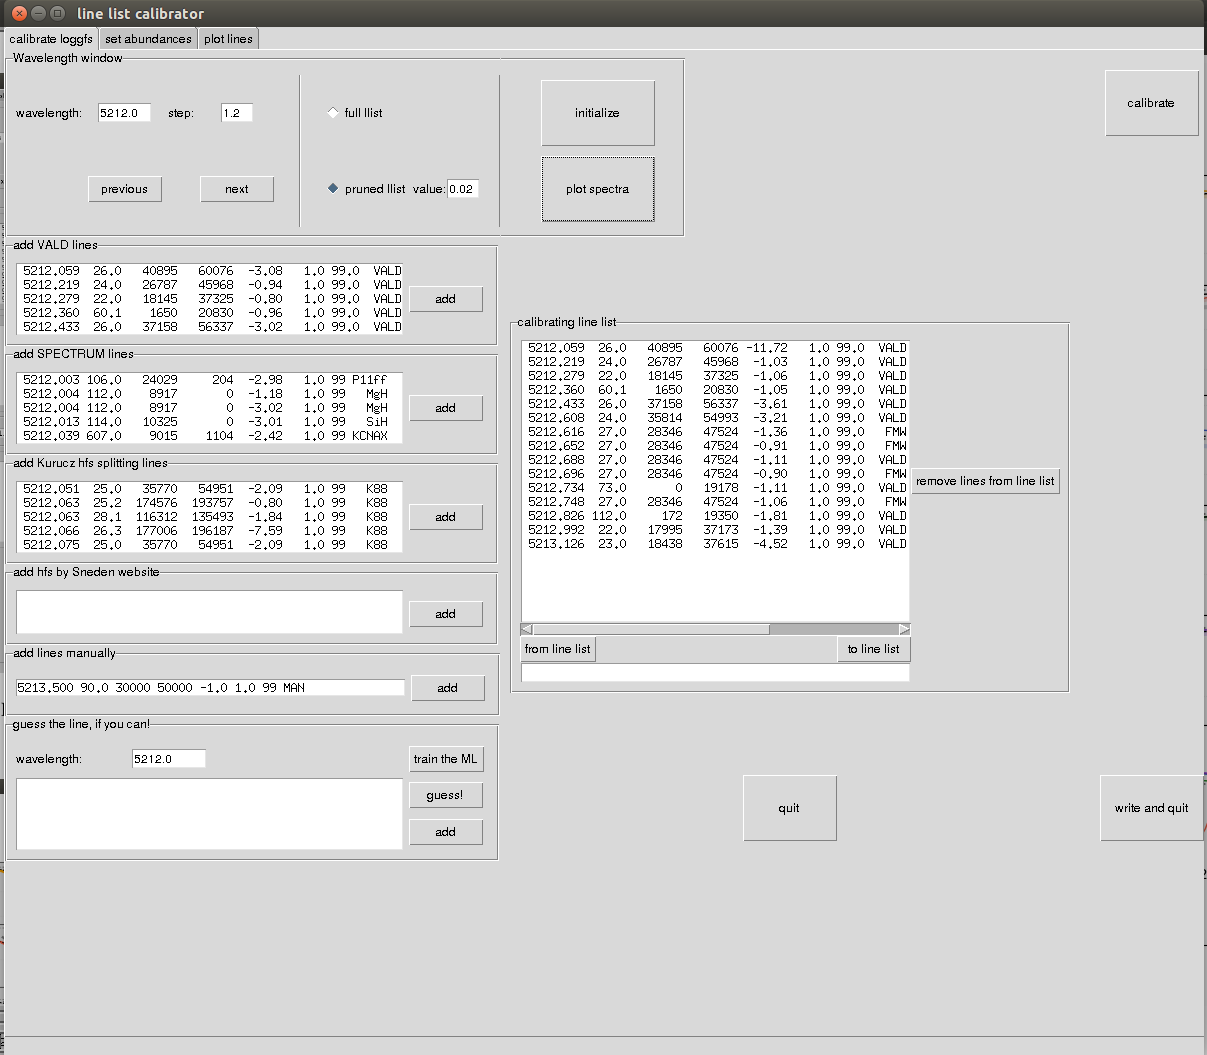
\includegraphics[width=12cm]{pics/calibrate_loggfs.png}
\caption{The oscillator strength (\loggf)s interface.}
\label{calibrate_loggfs}
\end{minipage}
\vskip 1cm
\begin{minipage}[t]{14cm}

%\begin{figure}[h]
\centering
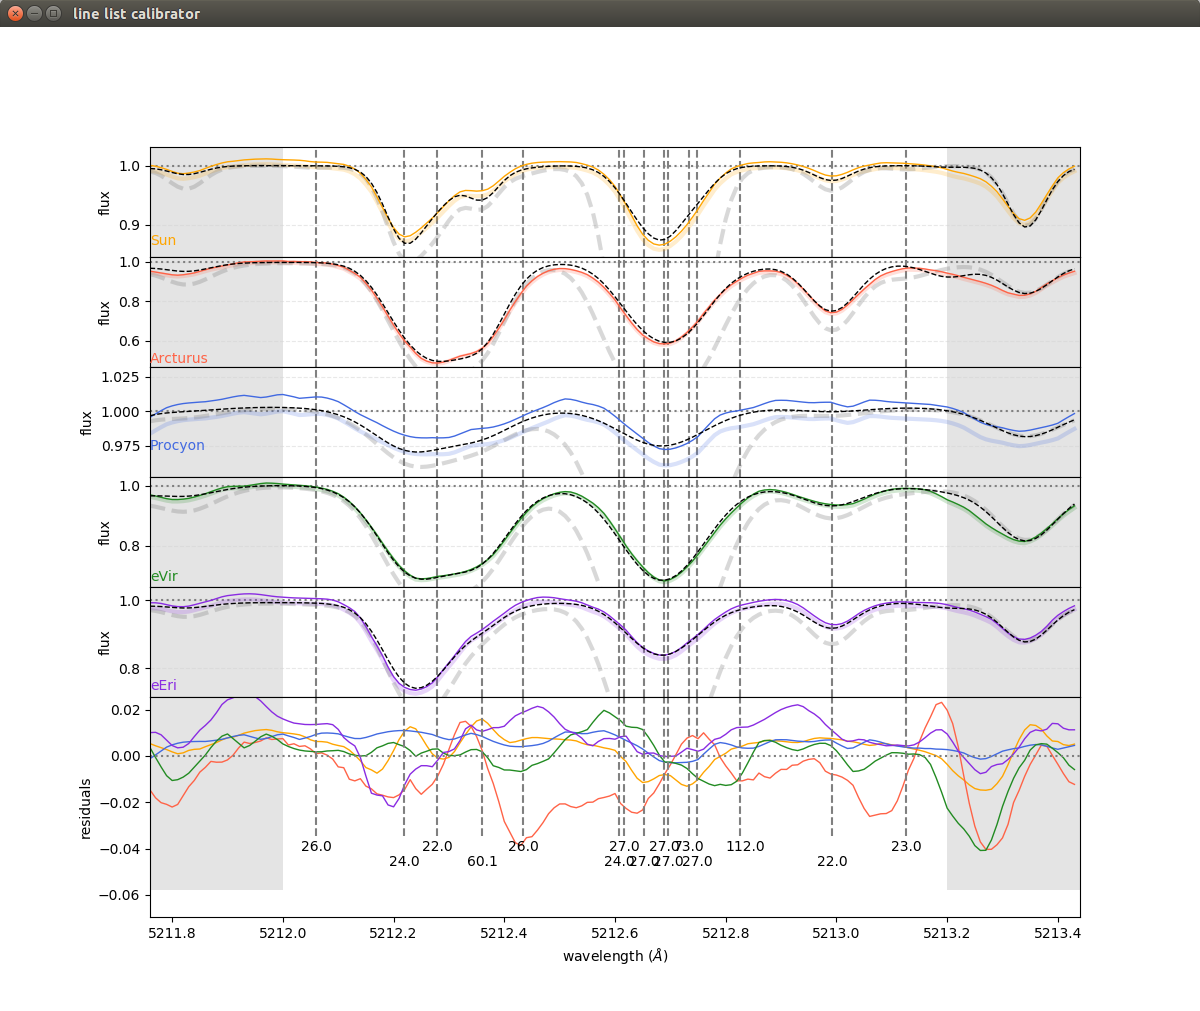
\includegraphics[width=12cm]{pics/plot_loggfs.png}
\caption{Plot window of loggfs calibration.}
\label{plot_loggfs}
\end{minipage}
\end{figure*}



%%%%%%%%%%%%%%%%%%%%%%%%%%%%%%%%%%%%%%

\subsection{The abundance calibration tab}\label{sec_abd_tab}

This window (see Fig.~\ref{calibrate_abundances}) has two frames:\\
\begin{itemize}
%
\item {\em elements to plot}: first, click on the button {\em show
elements},
then choose up to 4 elements by clicking on them. The button
{\em plot NEWRs} plots the NEWRs (Normalized Equivalent Width Residuals)
as a function of their EW in the graphical
window. The plot show the EWs distribution for each of the 5 standard stars
(see Fig.~\ref{plot_abundances}).
The user can set the {\em minimum purity} value 
of the lines to be shown in the plot\footnote{The definition 
of ``purity" has been given in Sec.3.4
of the paper Boeche, Vallenari, Lucatello, submitted 2020.}.
Clicking on the button {\em plot params check (MOOG like)} the user can
visualize the NEWRs of a choosen element as a function of excitation
potential, logarithm of the reduced EW, and wavelength $\lambda$, similarly
to what is done in MOOG (see Fig.~\ref{plot_abd_mooglike}).
%
\item{\em abundances to change}: here one can set the abundances for every
standard star. After the abundance setting the button {\em recompute NEWRs} must be
pressed in order to make the changes effective. After this, to see the
changes, press the button {\em plot NEWRs} again. {\bf Important suggestion}: if the
wavelength interval in calibration is large, the {\em recompute NEWRs}
button may take long time to return because
it synthesizes the whole wavelength interval for all the standard stars. A
more convenient way to do the same is teh following: set the elements abundance and press the button
{\em write the abd files} which only writes the files where the abundances
for the synthesis are stored. After that, run the {\tt
calibrator\_batch.py} which automatically re-calibrate the \loggf s with the
newly set abundances. Then, check the results with {\tt
calibrator\_routine.py}.\\

The user can add elements by editing the files atmospheres/star?.abd and
adding the wanted elements.
%
\end{itemize}



\begin{figure*}[h]
\begin{minipage}[t]{14cm}
\centering
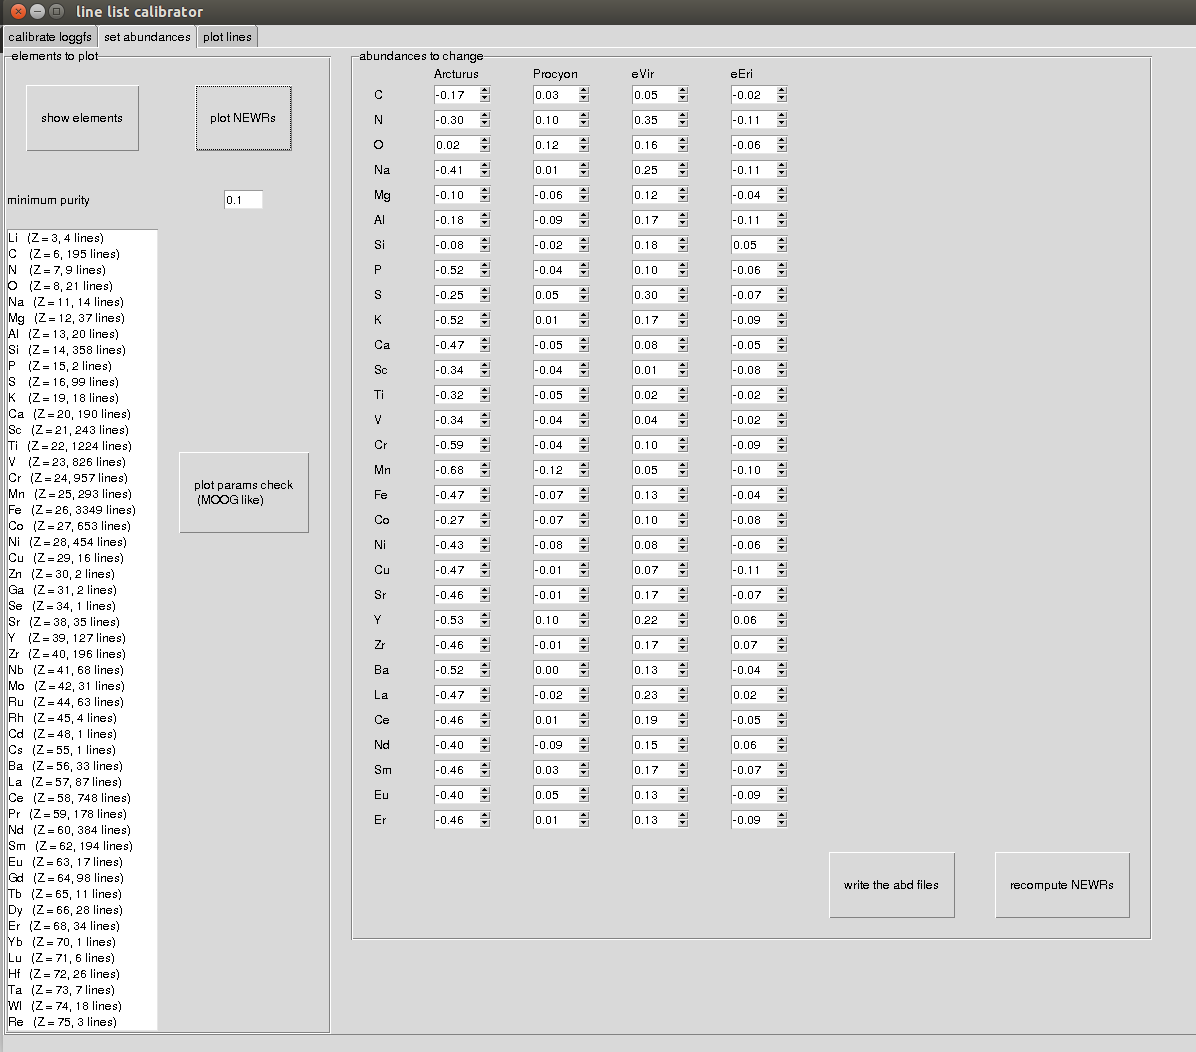
\includegraphics[width=12cm]{pics/calibrate_abundances.png}
\caption{The abundances interface.}
\label{calibrate_abundances}

\end{minipage}
\vskip 1cm
\begin{minipage}[t]{14cm}

\centering
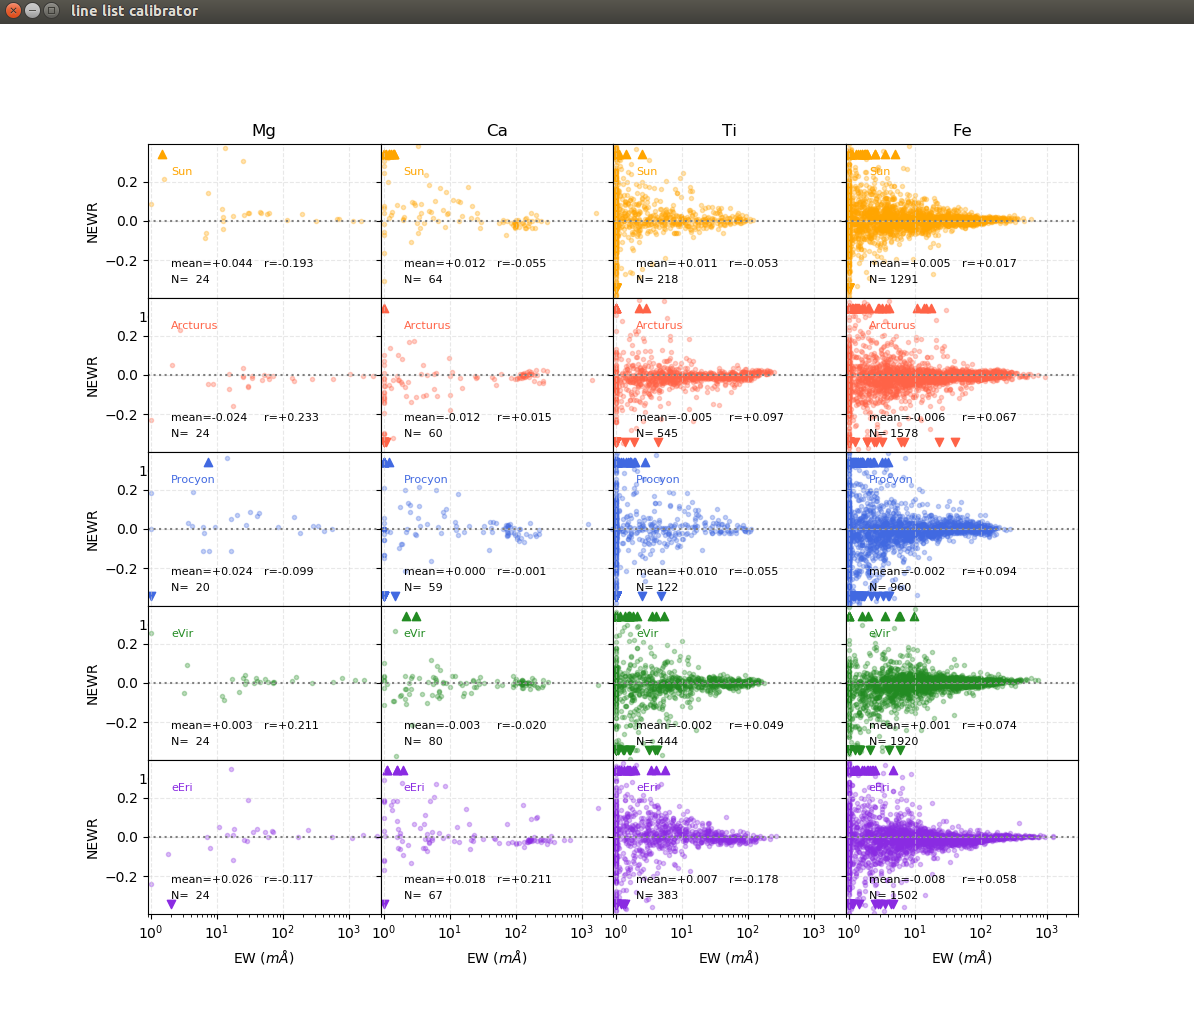
\includegraphics[width=12cm]{pics/plot_abundances.png}
\caption{The abundances plot window.}
\label{plot_abundances}
\end{minipage}
\end{figure*}

\begin{figure*}[h]
\centering
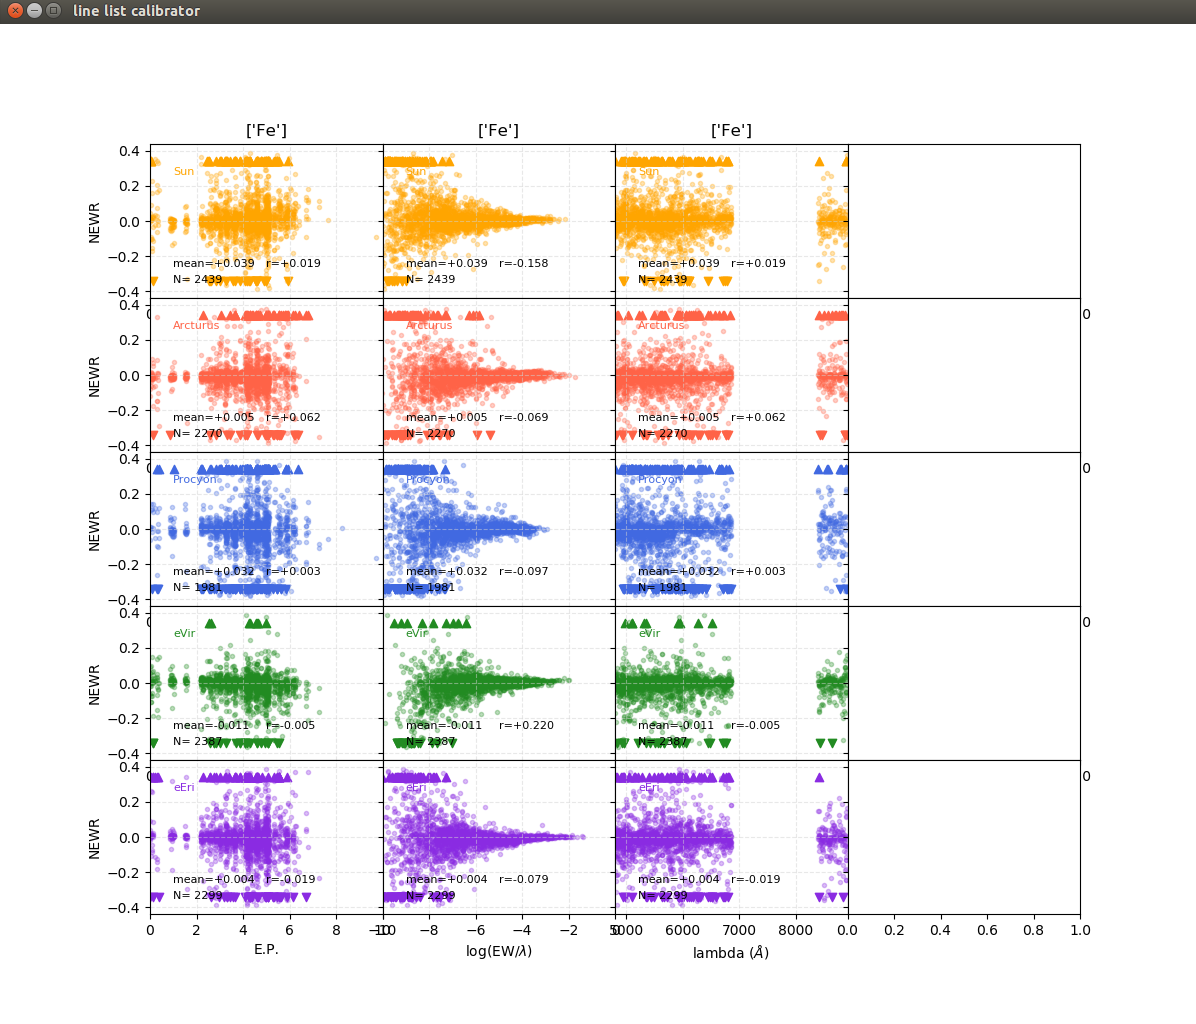
\includegraphics[width=12cm]{pics/plot_abd_mooglike.png}
\caption{The abundances plot window as MOOG would shows.}
\label{plot_abd_mooglike}
\end{figure*}

%%%%%%%%%%%%%%%%%%%%%%%%%%%%%%%%%


\subsection{The plot lines tab}
With this interface the user can visualize a specific line and, when
desired, calibrate the Van der Waals broadening parameter.
It contains two frames:\\
\begin{itemize}
%
\item {\em element lines to plot}: this is a useful tool to eye-check the lines by element. Press the button
{\em show elements} to see the element list and select one element per time.
Then press {\em initialize} and {\em plot} to see in the graphical window three lines of the
element per time. To move through all the lines of the chosen element, press the buttons
{\em next} or {\em previous} and the {\em plot}. The {\em wavelength} entry
takes as input the starting wavelength of the lines to be visualized. As
example, by putting 6000 only lines with wavelengths larger than 6000\AA\
will be proposed. This is
useful when there are many lines (thousands in the case of Fe) and one want
to move quickly to the redder region. With the entry {\em minimum EW} one can select the minimum EW that
the lines shown must have. Similarly does the {\em minim purity} entry.
%
\item {\em calibrate Van der Waals parameter}: the window shows the atomic
parameters of the three lines plotted in the graphical window. By clicking
on one of them, and then on the button {\em calibrate VdW}, the Van der Waals
fudge factor parameter given in SPECTRUM will be automatically adjusted to match at best
the line (using a $\chi$ square minimization process). 
By pressing {\em initialize} the newly computed VdW value will be shown and
by pressing {\em plot} the synthetic line with the new VdW value will be
plotted. The button {\em undo VdW} the VdW value is reported to its original
value.\\
If the user want to set the VdW value by hand, he/she can use the \loggf\ 
calibration interface and use the buttons {\em from line list} and  {\em to line
list} to edit any atomic parameter of the line.

%
\end{itemize}


\begin{figure*}[h]
\begin{minipage}[t]{14cm}
\centering
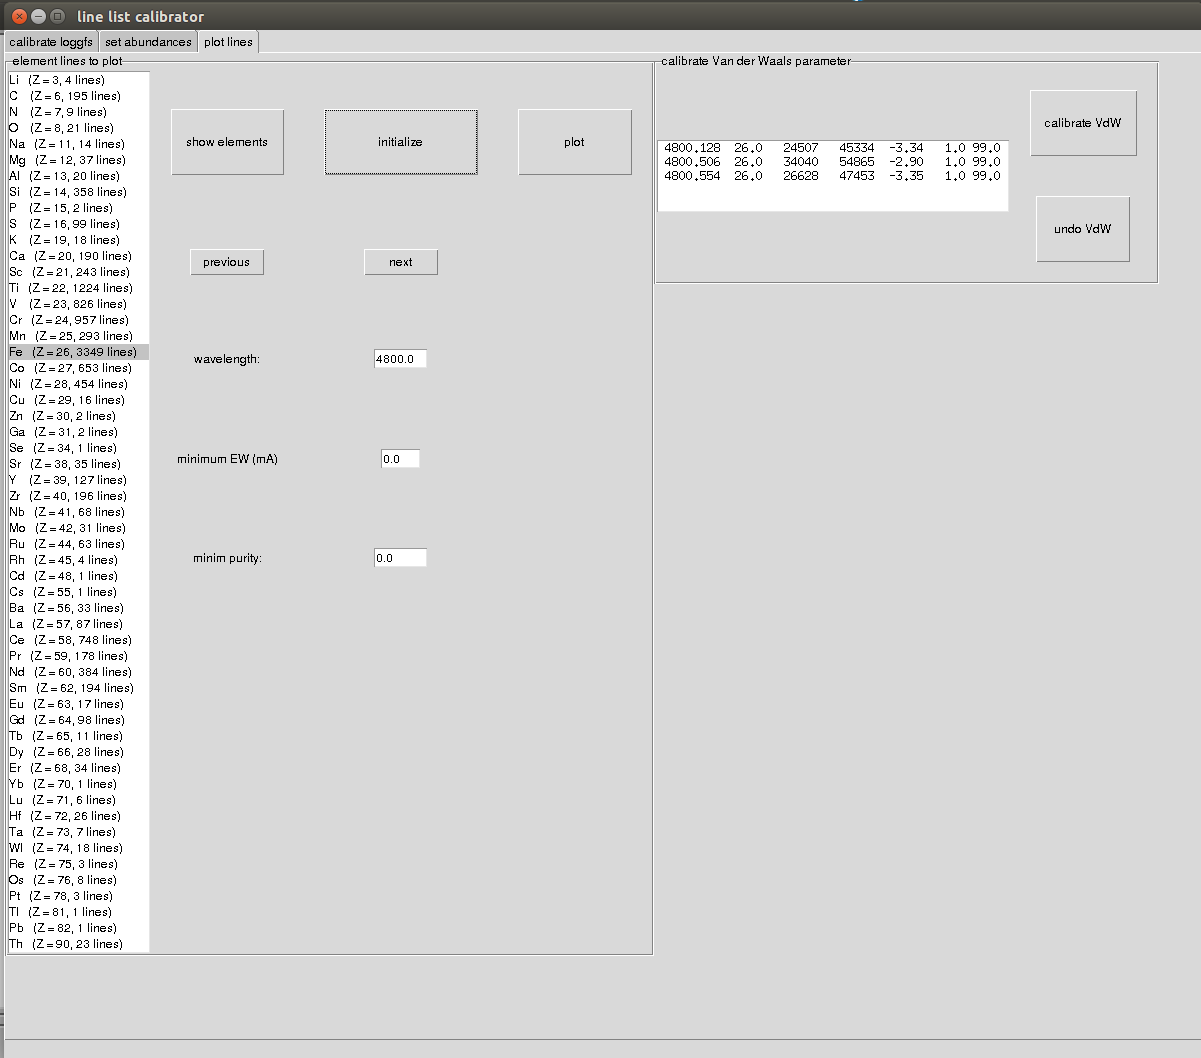
\includegraphics[width=12cm]{pics/plot_lines_tab.png}
\caption{The plot lines interface.}

\end{minipage}
\vskip 1cm
\begin{minipage}[t]{14cm}


\centering
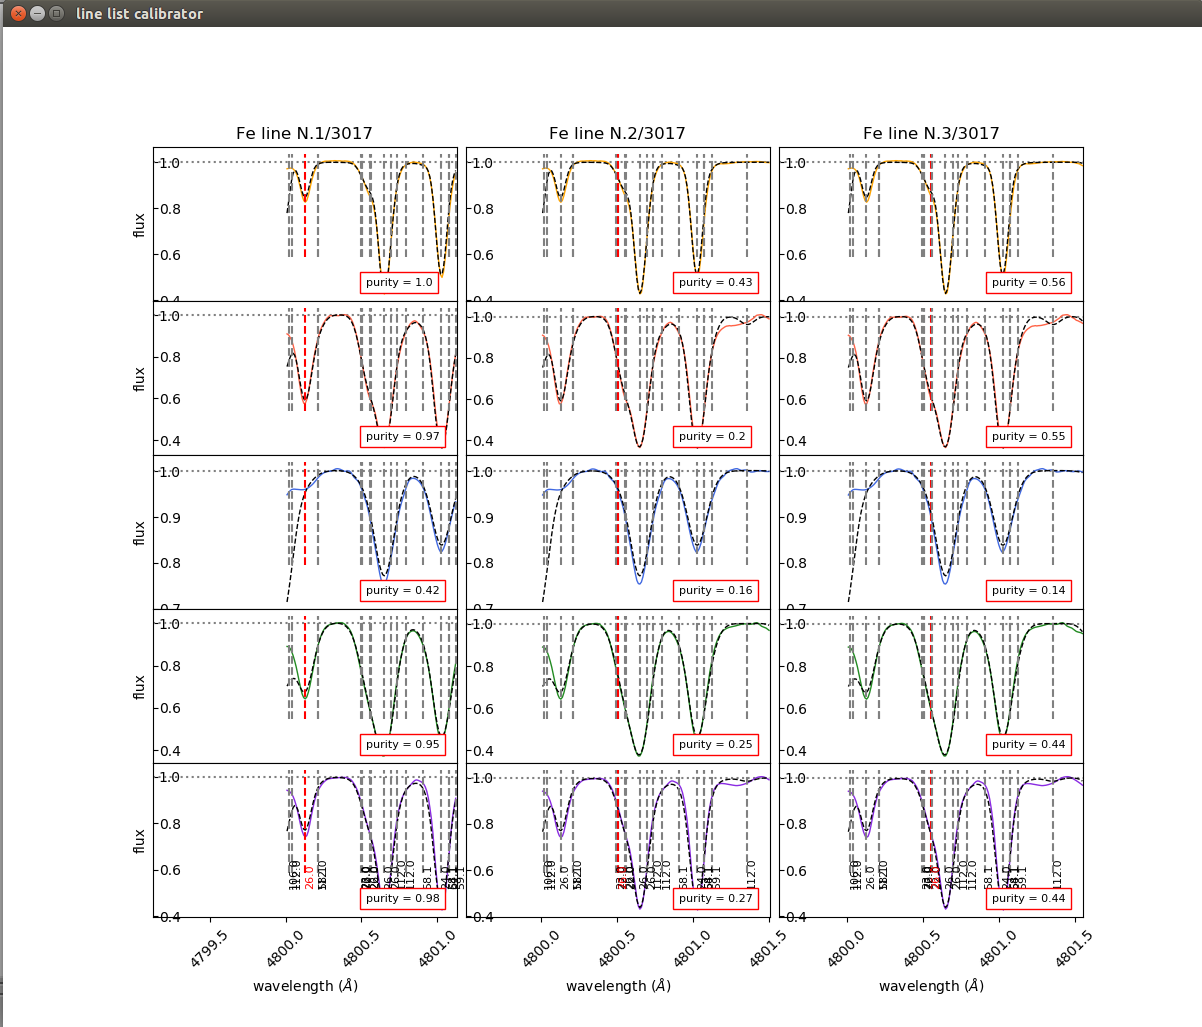
\includegraphics[width=12cm]{pics/plot_lines.png}
\caption{The plot lines interface.}
\end{minipage}
\end{figure*}



%%%%%%%%%%%%%%%%%%%%%%%%%%%%%%%%%%%%

\end{document}
